\documentclass[12pt]{article}

\usepackage{fullpage}
\usepackage[round]{natbib}
\usepackage{multirow}
\usepackage{booktabs}
\usepackage{graphicx}
\usepackage{float}
%\usepackage{../ltx/edcomms}
\usepackage{../ltx/setupComments}
\usepackage{hyperref}
\usepackage{geometry}
\usepackage{changepage}
\usepackage{adjustbox}
\usepackage{graphicx}
\usepackage[section]{placeins} % Prevents floats from floating across sections
\usepackage{tabularx}
\usepackage{amsfonts}
\usepackage{glossaries}
\usepackage{multirow} %% Used for Traceability matrix
%\usepackage{amssymb}
\newcounter{acnum}
\newcommand{\actheacnum}{AC\theacnum}
\newcommand{\acref}[1]{AC\ref{#1}}

\newcounter{ucnum}
\newcommand{\uctheucnum}{UC\theucnum}
\newcommand{\uref}[1]{UC\ref{#1}}

\newcounter{mnum}
\newcommand{\mthemnum}{M\themnum}
\newcommand{\mref}[1]{M\ref{#1}}
\makeglossary
\begin{document}

\title{\vspace*{3cm} Module Guide for ECA Rules for Ampersand} 
\author{Yuriy Toporovskyy (toporoy)\\ Yash Sapra (sapray) \\ Jaeden Guo (guoy34)}
%%Yuriy Toporovskyy (toporoy) \\ Yash Sapra (sapray) \\ Jaeden Guo (guoy34)}
\date{February 24th,\ 2016} 


\maketitle
\newpage
\vspace*{1cm}
\begin{table}[ht!]\begin{center}
        \caption{Revision History}  
        \begin{tabular}{|c|c|c|}\hline
            \textbf{Author} & \textbf{Date} & \textbf{Comments} \\\hline 
            Yash Sapra & 24 / 02 / 2016 & Initial draft\\\hline
	 Jaeden Guo & 27/ 02 / 2016 & Update and merge \\\hline
        \end{tabular}
    \end{center}\end{table}
\newpage

\tableofcontents

\newpage

\section{Introduction}
%TODO: edit for grammar, spelling, context, flow, watch for contractions
\subsection{Description}
This document follows the principle set by Parnas and Clements\citep{fakeIt}. 
EFA is currently in development where changes occur frequently, a 
commonly accepted practice for this situation is to decompose modules based on 
the principle of abstraction, where unnecessary information in hidden for the 
benefit of designers and maintainers\citep{modStruct,Parnas1972}.
 
Our design follows the principles laid out by \citep{modStruct}, as follows:
\begin{itemize}
\item Unnecessary design details are omitted for simplicity
\item Each module is broken down based on hierarchy with no overlap of functionality
\item All our modules are Open Modules i.e they are available for extension in the future
\item Reference material are provided for external libraries
%% but details of its use will not be provided within the module break-down
\end{itemize}

The language of implementation is Haskell.

\subsection{Scope}
The purpose of this document is to outline the implementation details of the EFA project described in the Problem Statement.
%The document outlines the design decision for the EFA project. 
EFA is responsible for generating SQL Statements from ECA rules that will 
be used to fixed any data inconsistencies in the Ampersand Database. 
The document will serve as a referral document for future Software Development in the Ampersand project.

\subsubsection{Intended Audience}
This document is designed for:
\paragraph{New project members:}
This document designed to be a guide to introduce new Ampersand users to EFA 
(ECA rules for Ampersand). It provides a basic structure that allows 
individuals to quickly access what they are looking for.
   
\paragraph{Maintainers \& Designers:} The structure of this module guide will 
help maintainers rationalize where changes should be made in order to 
accomplish their intended purpose. Furthermore, the design document will act as 
a guide to EFA for future designers of Ampersand.

\section{Anticipated and Unlikely Changes}
\subsection{Anticipated Changes}
It is likely that EFA will require changes to the front-end interface and an 
addition that will connect the front-end interface to back-end functions, which 
will give the user more control. In addition, ECA rules are not static and may 
change over time, if changes do take place those changes will need to be 
incorporated into EFA's future versions. 

Thus far anticipated changes include:

\begin{description}
    \item[AC1:] New front-end interface.
    \item[AC2:] Addition or elimination of ECA rules.
    \item[AC3:] The algorithm used for EFA.
    \item[AC4:] The format of output.
    \item[AC5:] The format of input parameters.
    \item[AC6:] Integration of front-end interface to back-end modules.
    \item[AC7:] Testing for individual modules and internal systems.
    
\end{description}

\subsection{Unlikely Changes} 

These unlikely changes include the things that will remain unchanged in the 
system, and also changes that would not affect EFA. 

\begin{description}
    \item[UC1:] There will always be a source of input data external to the 
    software.
    \item[UC2:] Results will always be provably correct.
    \item[UC3:] Output data must exist.
    \item[UC4:] The implementation language must be the same as that which is 
    used for building the Ampersand system.
    \item[UC5:] The format of initial input data and associated markers for 
    data association.
    \item[UC6:] Type of output data will always be a SQL procedure.
\end{description}

\section{Module Hierarchy}
This section provides an overview of the module design. Modules are decomposed 
based on their hierarchy from top to bottom. The modules are broken down into 
three sections, the first section consists of the main module used for EFA, 
the second section contains support modules and finally the last section
contains external libraries.

\begin{figure}
    \centering
    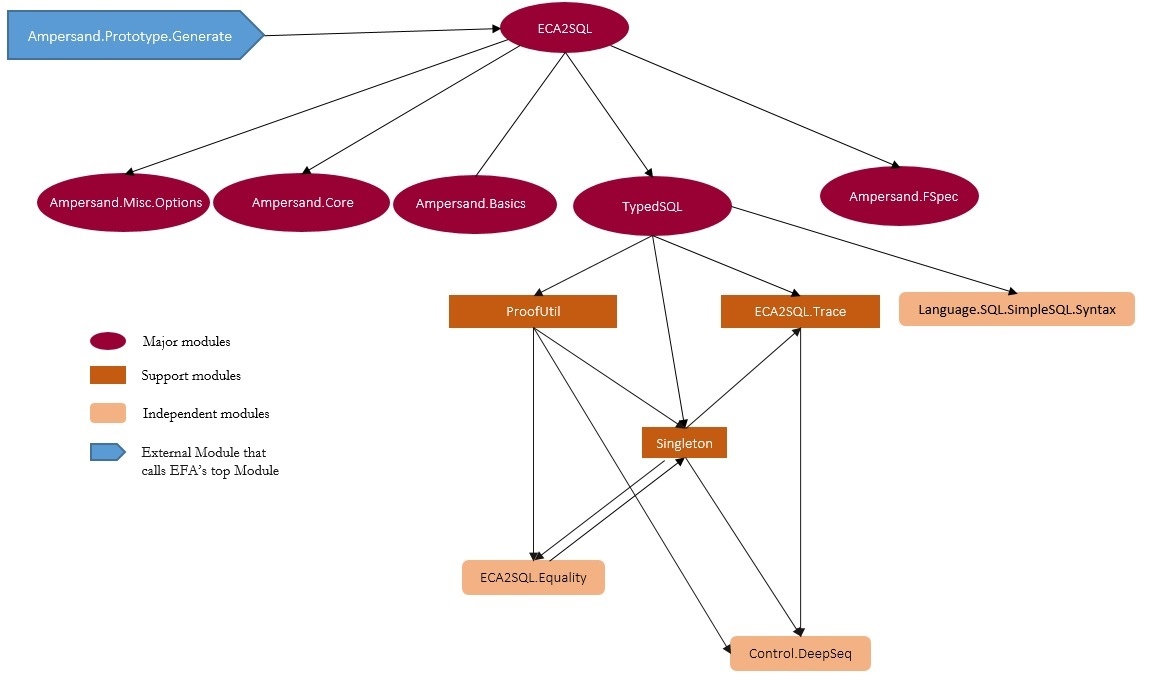
\includegraphics[width=0.95\textwidth]{../figures/depent_tree}
    \caption{Dependency graph of EFA modules}~\label{fig:figure1}
\end{figure}

%%%%%%%%%%%%%%%%%%%%%
%%% Section - System Architecture %%%%%
%%%%%%%%%%%%%%%%%%%%%
\newpage
\section{System Architecture} \label{SystemArch}

\subsection{Key Algorithm}
The key Algorithm for the EFA project is AMMBR \cite{AMMBR}. AMMBR is a method that allows organization to build information systems that comply to their business requirements in a provable manner. This Algorithm is implemented in Ampersand and is responsible for translating the business requirements into ECA rules. These ECA rules contain information on how to fix any data violation and are translated into SQL in our EFA project.

\subsection{Communication Protocol}
The EFA implementation needs to communicate with the front end to be able to run the generated SQL when a violation occurs. 
	\begin{itemize}
		\item \textbf{Old communication protocol -  PHP engine} \newline
			In in existing version, Ampersand depends on PHP code to run the generated SQL on the database. However this comes at the cost of human intervention and maintenance cost for the development. 
		\item \textbf{New Communication protocol - Stored Procedures} \newline
			The developments teams of EFA has come to a conclusion that the best way of communicating with the front-end will be to use Stored Procedures\cite{SP}. The Stored Procedures provide the extra benefit of query optimization at compile time which results in better performance. While this is a suggested change, it will require changes to the existing Ampersand software in order to successfully implement this idea. This is an anticipated change and will be implemented in the near future.
			
	\end{itemize}

\subsection{Error handling}
Most of the error handling is done by the underlying Ampersand software. Any human errors (syntactic or semantical) in the input ADL file are handled during the generation of the ECA. The resulting ECA rules which are fed into the EFA project are provably correct. The language of implementation (i.e Haskell) guarantees type level correctness of the EFA project at compile time. 
\newline
If any error occurs during runtime, the state of the database will be checked before and after the SQL statement is run. In case of an inconsistency in the data, the SQL \textbf{rollback} command will be issued that will change the database to its previous state. In such a scenario, the user will be notified about the event and can take necessary actions to fix the issue. 

\subsection{Main Module}

%% ------------------------------M1: ECA2SQL -------------------------------%%
{\setlength{\tabcolsep}{6pt} 
    \begin{tabularx}{\textwidth}{>{\bfseries}m{3cm}X}
        M1 & eca2SQL \\ 
        \midrule 
        Main function & eca2SQL
        \\  Input & Options, FSpec, ECARule
        \\  Output & Doc
        \\	Services & Produces the final product by using supporting modules 
        as tools in translating ECA rules to SQL statements which can be 
        applied to a database.
        \\     
         \vspace{12pt}
     \end{tabularx}
\\
\underline{Internal Description}\\ \\
eca2SQL :: Options $\rightarrow$ FSpec $\rightarrow$ ECArule $\rightarrow$ Doc

%% ------------------------------M2: TypedSQL -------------------------------%%
\subsection{Support Modules}

{\setlength{\tabcolsep}{6pt} 
    \begin{tabularx}{\textwidth}{>{\bfseries}m{4cm}X}
        M2 & eca2SQL \\ 
        \midrule       
        \\  Requires Modules & ProofUtils, Trace, Singleton
        \\	Services & Implements a type language for SQL through pattern 
        matches where the representation of SQL references types which can 
        appear in SQL statements. Contains Base which implements a typed SQL query 
        language and a type SQL statement.
        \\         
        \vspace{12pt}
    \end{tabularx} 


\setlength{\parindent}{0pt}
\underline{Internal Description}\\

Read as: \textit{function: input $\rightarrow$ input2 $\rightarrow$ 
output}\newline

Where a function may require multiple inputs of different types to produce the 
necessary output type.\\

\textit{function (type and value level): (x:A) $\rightarrow$ output}
This indicates the function of a certain type and its value level, this is seen 
on SQL types. (x:A) is used to indicate a variable x of type A (e.g. x=9, (x:A) 
is a type of integer). (function::) is used to define a function and its input 
types 



\newglossaryentry{N}{name=N, description= $\mathbb{N}$ represents 
    the 
    set of natural numbers}

 (:::) : Symbol $\rightarrow$ SQLType $\rightarrow$ SQLRecLabel \\
 
 SQLSizeVariant : Kind \\
 SQLSmall, SQLMedium, SQLNormal, SQLBig :SQLSizeVariant \\ \\
 
 SQLSign : Kind \\
 SQLSigned, SQLUnsigned : SQLSign  \\
 
 SQLNumeric : Kind \\
 SQLFloat, SQLDouble : SQLSign $\rightarrow$ SQLNumeric \\
 
 SQLInt : SQLSizeVariant $\rightarrow$ SQLSign $\rightarrow$ SQLNumeric \\
 SQLRecLabel : Kind \\

 SQLType : Kind \\
 SQLBool, SQLDate, SQLDateTime, SQLSerial : SQLType \\
 
 SQLNumericTy : SQLNumeric $\rightarrow$ SQLType  \\
 SQLBlob : SQLSign $\rightarrow$ SQLType \\
 
 SQLVarChar : N $\rightarrow$ SQLType 
 SQLRel : SQLType $\rightarrow$ SQLType \\
 
 SQLRow : [SQLRecLabel] $\rightarrow$ SQLType 
 SQLVec : [SQLType]$\rightarrow$ SQLType \\
 
 SQLRef, SQLUnit: SQLType \\
 SQLRefType: Kind\\
 
 SQLMethod: [SQLType] $\rightarrow$ SQLType $\rightarrow$ SQLRefType \\
 SQLVal: SQLType $\rightarrow$ Type \\
 
 SQLScalarVal: IsScalarType a $\equiv$ True $\rightarrow$ Sm.ValueExpr 
 $\rightarrow$ SQLVal a \\
 SQLQueryVal: IsScalarType a $\equiv$ False $\rightarrow$ Sm.QueryExpr 
 $\rightarrow$ SQLVal a \\
 
 SQLValSem: SQLRefType $\rightarrow$ Type\\

 
 Ty: SQLType $\rightarrow$ SQLRefType \\

 IsScalarType: SQLType $\rightarrow$ Bool \\
 isScalarType: (x:SQLType) $\rightarrow$ IsScalarType x \\
 IsScalarTypes: [SQLType] $\rightarrow$ Bool \\
 isScalarTypes: (X:[SQLType]) $\rightarrow$ IsScalarTypes x \\
 
 typeOf: SQLVal a $\rightarrow$ a \\
 argOfRel: SQLRel a $\rightarrow$ a\\
 
 Unit: SQLValSem SQLUnit\\
 Val:: SQLVal x $\rightarrow$ SQLValSem ('Ty x)
 
 

%% ------------------------------M3: Equality -------------------------------%%
{\setlength{\tabcolsep}{6pt} 
    \begin{tabularx}{\textwidth}{>{\bfseries}m{4cm}X}
        M3 & Equality \\ 
        \midrule
        
        Contains functions  &  not, cong, elimNeg and more
        \\	Services &  The module contains utility functions that are being used in the Singletons and Utils module to provide type 		level security for the TypedSQL with an aim to make it total. It implements a primitive strict negation type, a strict decidable equality type,  and various equality proof function
        \\       
        \vspace{12pt}
    \end{tabularx}
    \vspace{3em}
%% ------------------------------M4: Singleton -------------------------------%%
{\setlength{\tabcolsep}{6pt} 
    \begin{tabularx}{\textwidth}{>{\bfseries}m{4cm}X}
        M4 & Singleton \\ 
        \midrule
        
        Main function  &  No functions exported
        \\	Services &  Singletons contains an implementation of singletons (types which are inhabited by precisely one value)
  in a kind-generic way. This is used in contrast to the `singletons' package which makes heavy use of 
  Template Haskell. To avoid this massive pitfall, we have reimplemented singletons without Template Haskell.
        \\       
        \vspace{12pt}
    \end{tabularx}\vspace{3em}
%% ------------------------------M5: Utils -------------------------------%%
{\setlength{\tabcolsep}{6pt} 
    \begin{tabularx}{\textwidth}{>{\bfseries}m{4cm}X}
        M5 & Utils \\ 
        \midrule
        
        Main function  & 
        \\	Services &  The module also contains some utility functions used by the ECA2SQL module
        \\       
        \vspace{12pt}
    \end{tabularx}\vspace{3em}
%% ------------------------------M6: Trace -------------------------------%%
{\setlength{\tabcolsep}{6pt} 
    \begin{tabularx}{\textwidth}{>{\bfseries}m{4cm}X}
        M6 & Trace \\ 
        \midrule
        
        Main function  &  getTraceInfo 
        \\	Services &  The modules contains support for tracing back the ECA rule. It implements a proper error message (with line numbers and function name). Tracing is used for development and debugging purpose
        \\       
        \vspace{12pt}
    \end{tabularx}\vspace{3em}
%% ------------------------------M7: Combinators------------------------------%%
{\setlength{\tabcolsep}{6pt} 
    \begin{tabularx}{\textwidth}{>{\bfseries}m{5cm}X}
        M7 & Combinators \\ 
        \midrule
        
        Main function  & No functions exported
        \\	Services &  This module contains Combinatory Logic for our TypedSQL module. The module defines SQL primitives such as AND, OR, NOT and the primitive SQL functions such as the EXISTS, GROUP BY, SORT BY.
        \\       
        \vspace{12pt}
    \end{tabularx}\vspace{3em}
%% ----------------------------- M8: Pretty    ------------------------------%%
    {\setlength{\tabcolsep}{6pt} 
        \begin{tabularx}{\textwidth}{>{\bfseries}m{5cm}X}
            M8 & Pretty \\ 
            \midrule
            
            Main function  & eca2PrettySQL
            \\	Services &  The module contains a pretty printer for the Typed SQL types. The intended purpose of this pretty printer is to produce human-readable SQL Statements.
            \\       
            \vspace{12pt}
        \end{tabularx}\vspace{3em}
\underline{Internal Description}\\ \\
eca2PrettySQL :: Options $\rightarrow$ FSpec $\rightarrow$ ECArule $\rightarrow$ Doc

\section{Module Decomposition} \label{SecMD}
Modules are located in their respective subsections (i.e. main module, support 
modules and external library modules). Each module is decomposed based on their 
use while hiding implementation details. 
\\ \newline
\textit{Please see glossary for math references and clarification of uncommon 
terms}

        
\subsection{External Libraries}
The EFA project depends on the following Libraries 
\begin{description}
	\item \textbf{Ampersand Core Libraries} \newline
		The EFA project depends on the Ampersand software for the definition of core Data Structures, i.e FSpec (which contains the definition to the underlying ECA rules). EFA also maintains the relational schema of the input and hence imports Ampersand's existing functions to fetch the table declarations while generating SQL Statements for the ECA rules. AMMBR \cite{AMMBR} which is the key algorithm responsible for translating business requirements into ECA rules is an intergral part of Ampersand.
	\item \textbf{Simple-sql-parser} \newline
		The pretty printer of the EFA project depends directly on this library for pretty printing the SQL statements in the console. This is important from a development and debugging perspective.\cite{simple-sql}
	\item \textbf{wl-pprint} \newline
		The wl-pprint library\cite{wl-pprint} is a pretty printer based on the pretty printing combinators described by Philip Wadler (1997). EFA uses this library in combination with the simple-sql-pretty to output the SQL statements in a human readable format.
	\item 
\end{description}

\section{Traceability Matrix} \label{SecTM}

%% TODO : Fix position
Note : The traceability matrix is based on test plan submitted by the EFA team. Removing test cases 11,12,13 which are not feasible at this point. These test cases will be removed from the Test plan in the next update.

\begin{table}[]
\caption{Traceability Matrix for the EFA Project}
\label{traceMatrixl}
\begin{tabular}{llllllll}
\multicolumn{1}{c}{}                                                   & \multicolumn{7}{l}{Requirements}  \\
\multirow{11}{*}{\begin{tabular}[c]{@{}l@{}}Test\\ Cases\end{tabular}} &     & F1 & F3 & F4 & F6 & N1 & N2 \\
                                                                       & T1  & X  &    &    &    &    &    \\
                                                                       & T2  & X  &    &    &    &    &    \\
                                                                       & T3  & X  &    &    &    &    &    \\
                                                                       & T4  & X  &    &    &    &    &    \\
                                                                       & T5  & X  & X  &    &    &    &    \\
                                                                       & T6  &    & X  &    &    &    &    \\
                                                                       & T7  &    &    & X  &    &    &    \\
                                                                       & T8  &    &    &    & X  & X  &    \\
                                                                       & T9  &    &    &    &    &    & X  \\
                                                                       & T10 &    &    &    & X  &    &   
\end{tabular}
\end{table}


%%%\section{Use Hierarchy Between Modules} \label{SecUse}





%\section*{References}
\clearpage
\printglossaries
\bibliographystyle{plain}
\bibliography {docDesign}

\end{document}